\documentclass[prc]{revtex4}
% The file compiles both with pdflatex and with latex + dvips + ps2pdf.
% All figures are drawn with TikZ; no PostScript-only packages are needed.
\usepackage{graphicx}
\usepackage{mathrsfs} \usepackage{amsfonts}
\usepackage{amsmath} \usepackage{amssymb}
\usepackage[T1]{fontenc}
\usepackage{hyperref}
\usepackage{dcolumn}% Align table columns on decimal point
\usepackage{bm}% bold math

\usepackage{tikz}
\usetikzlibrary{decorations.markings,arrows.meta,shapes.misc}
\tikzset{
  gdiag/.style={scale=0.95},
  gpart/.style={thick,postaction={decorate},
    decoration={markings,mark=at position 0.56 with
      {\arrow{Stealth[length=6pt,width=5pt]}}}},
  ghole/.style={thick,postaction={decorate},
    decoration={markings,mark=at position 0.56 with
      {\arrowreversed{Stealth[length=6pt,width=5pt]}}}},
  gint/.style={dashed,thick},
  gdot/.style={circle,fill,inner sep=1.3pt},
  gcross/.style={cross out,draw,thick,minimum size=6pt,inner sep=0pt},
  glab/.style={font=\small},
  occ/.style={circle,fill,draw,inner sep=0pt,minimum size=3mm},
  emp/.style={circle,draw,fill=white,inner sep=0pt,minimum size=3mm}}

\newcommand{\One}{\hat{\mathbf{1}}} \newcommand{\eff}{\text{eff}}
\newcommand{\Heff}{\hat{H}_\text{eff}}
\newcommand{\Veff}{\hat{V}_\text{eff}}
\newcommand{\braket}[1]{\langle#1\rangle}
\newcommand{\Span}{\operatorname{sp}}
\newcommand{\tr}{\operatorname{trace}}
\newcommand{\diag}{\operatorname{diag}}
\newcommand{\bra}[1]{\left\langle #1 \right|}
\newcommand{\ket}[1]{\left| #1 \right\rangle} \newcommand{\element}[3]
           {\bra{#1}#2\ket{#3}}

\newcommand{\normord}[1]{ \left\{#1\right\} }

% Sub-items of an exercise are labelled (i), (ii), ...
\renewcommand{\labelenumii}{(\roman{enumii})}

\begin{document}

\begin{center}
{\LARGE\bf
Second midterm FYS4480 – Quantum mechanics for many-particle systems, deadline November 23, at midnight (23:59). This midterm counts 25$\%$ of the final grade. Total score:100 points.}
\end{center}
\begin{center}
% List of all institutions:
\centerline{{\small Department of Physics, University of Oslo, Norway}}
\end{center}


This midterm is a continuation of the first midterm. We use the same
simplified Hamiltonian, consisting of an unperturbed Hamiltonian and a
so-called pairing interaction term. It is a model which to a large
extent mimics some central features of atomic nuclei, certain atoms
and systems which exhibit superfluidity or superconductivity. In the
first midterm we studied this model with full configuration
interaction (FCI) theory, which provided us with the exact answer,
with Hartree-Fock (HF) theory and with the density matrix
renormalization group (DMRG). The topic of this midterm is many-body
perturbation theory (MBPT), with the pairing model as our example
throughout.

The midterm is divided into four parts. In Part I we derive
Rayleigh-Schr\"odinger perturbation theory and the wave operator, and
compare the wave operator to first order with the wave function from
the exact diagonalization. In Part II the energy to third order in
the interaction is represented by diagrams; we find the diagrams which
are relevant for the pairing model and study how a Hartree-Fock
calculation affects the diagrams of perturbation theory. In Part III
we discuss how diagrams are computed efficiently, in a basis of Slater
determinants and in the single-particle basis, and you write a program
which computes the energy to second and third order. In Part IV all
results are compared with those of the first midterm, that is with
FCI, Hartree-Fock and the DMRG. You will need your programs and
results from the first midterm.

Several of the exercises look at the same quantities from different
angles, through diagrams, through matrices and in a program. You may
reuse your results and refer to an earlier exercise instead of
repeating a derivation or a figure.

The relevant background is the chapter on many-body perturbation
theory in the lecture notes, together with the lectures and slides of
weeks 44--46.

We repeat first the definition of the Hamiltonian and of the
single-particle basis from the first midterm. Thereafter we remind you
about the Hamiltonian matrix for a system with no broken pairs, define
the notation, and present the various exercises.


The Hamiltonian acting in the complete Hilbert space (usually infinite
dimensional) consists of an unperturbed one-body part, $\hat{H}_0$,
and a perturbation $\hat{V}$.

We limit ourselves to at most two-body interactions, our Hamiltonian
is then represented by the following operators
\[
\hat{H} = \sum_{\alpha\beta}\langle \alpha |h_0|\beta\rangle
a_{\alpha}^{\dagger}a_{\beta}
+\frac{1}{4}\sum_{\alpha\beta\gamma\delta}\langle \alpha\beta|
V|\gamma\delta\rangle
a_{\alpha}^{\dagger}a_{\beta}^{\dagger}a_{\delta}a_{\gamma},
\]
where $a_{\alpha}^{\dagger}$ and $a_{\alpha}$ etc.~are standard
fermion creation and annihilation operators, respectively, and
$\alpha\beta\gamma\delta$ represent all possible single-particle
quantum numbers.  The full single-particle space is defined by the
completeness relation $\hat{{\bf 1}} = \sum_{\alpha
  =1}^{\infty}|\alpha \rangle \langle \alpha|$.  In our calculations
we will let the single-particle states $|\alpha\rangle$ be
eigenfunctions of the one-particle operator $\hat{h}_0$. Note that the two-body part of the Hamiltonian
contains anti-symmetrized matrix elements.


The above Hamiltonian acts in turn on many-body Slater determinants
$|\Phi_m\rangle$ constructed from the single-particle basis defined by
the one-body operator $\hat{h}_0$. In perturbation theory the space
spanned by the Slater determinants is divided in two. A model space
is defined by the projection operator
\[
\hat{P} = \sum_{m\in\mathcal{M}}|\Phi_m\rangle\langle\Phi_m|,
\]
where the sum runs over a chosen set $\mathcal{M}$ of Slater
determinants, and the rest of the space is defined by its complement
\[
\hat{Q}=\hat{{\bf 1}}-\hat{P},\qquad \hat{P}+\hat{Q}=\hat{{\bf 1}} ,
\]
which projects on all Slater determinants which are not in
$\mathcal{M}$. In this midterm the model space consists of one Slater
determinant only, the reference state $|\Phi_0\rangle$ defined below.


Our specific model consists of $L$ doubly-degenerate and equally
spaced single-particle levels labelled by $p=1,2,\dots,L$ and spin
$\sigma=\pm 1$. A single-particle state (spin-orbital) is thus labelled
by $p\sigma$, and each level holds at most two particles.  These states
are schematically portrayed in Fig.~\ref{fig:schematic}.

We write the Hamiltonian as
\[ \hat{H} = \hat{H}_0 + \hat{V} , \]
where
\[
\hat{H}_0=\xi\sum_{p\sigma}(p-1)a_{p\sigma}^{\dagger}a_{p\sigma}
\]
and
\[
\hat{V}=-\frac{1}{2}g\sum_{pq}a^{\dagger}_{p+}
a^{\dagger}_{p-}a_{q-}a_{q+}.
\]
Here, $H_0$ is the unperturbed Hamiltonian with a spacing between
successive single-particle states given by $\xi$, which we will set to
a constant value $\xi=1$ without loss of generality. The two-body
operator $\hat{V}$ has one term only. It represents the pairing
contribution and carries a constant strength $g$. The pairing
interaction is attractive for $g>0$.

The indices $\sigma=\pm$ represent the two possible spin values. The
interaction moves a pair of particles with opposite spins from one
level $q$ to a level $p$. It never breaks a pair: the number of
particles which are not paired (the seniority) is conserved, and a
state with no broken pairs is coupled only to other states with no
broken pairs. A single application of $\hat{V}$ moves one pair. For a
system of four particles, the rightmost state in
Fig.~\ref{fig:schematic}, where one of the pairs has been moved to the
level $p=9$ and the other to the level $p=7$, is therefore reached
from the leftmost state by two applications of $\hat{V}$. The two
states in the middle contain broken pairs and cannot be reached from
the leftmost state with the present model.

The leftmost state in Fig.~\ref{fig:schematic}, with the two lowest
levels filled, is our reference state. The spin-orbitals which are
occupied in the reference state are called hole states, and all other
spin-orbitals are called particle states.

In our model we have kept both the interaction strength and the
single-particle level as constants.  In a realistic system like an
atom or the atomic nucleus this is not the case.


\begin{figure*}[htbp]
\centering
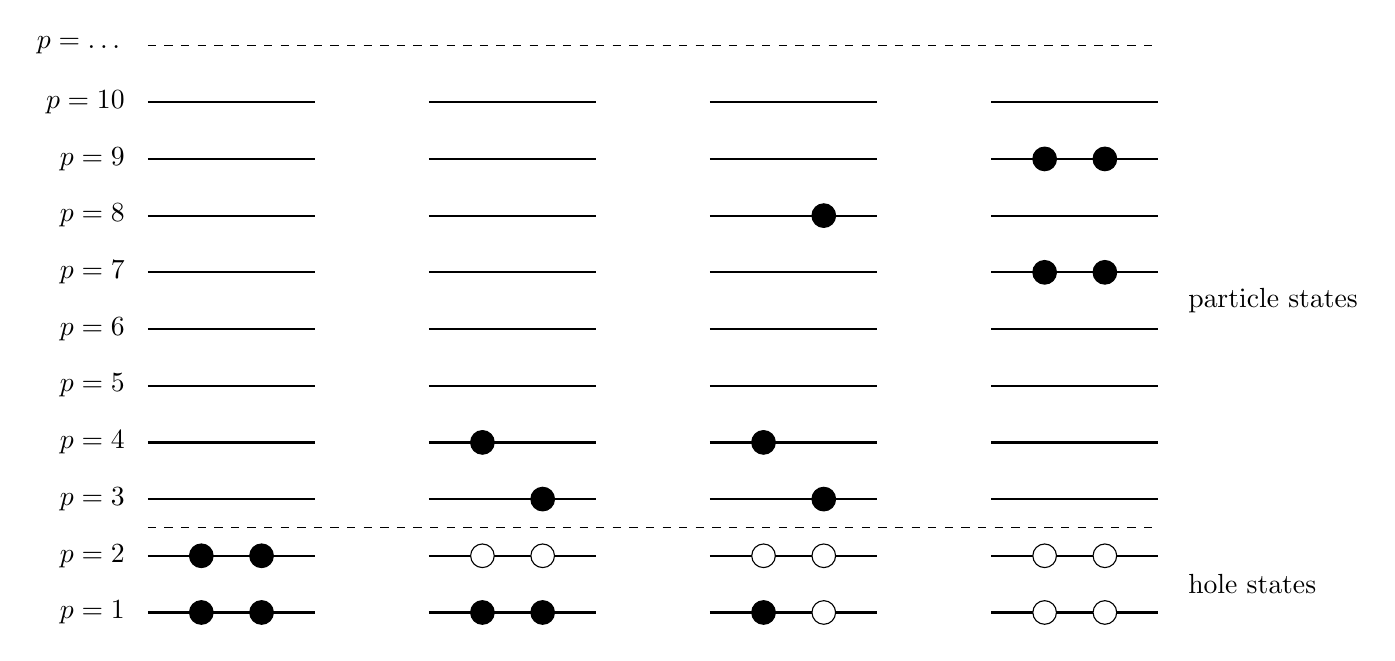
\begin{tikzpicture}[x=0.85cm,y=0.72cm]
  % the levels
  \foreach \p in {1,...,10} {
    \node[left] at (-0.2,\p) {$p=\p$};
    \foreach \x in {0,4.2,8.4,12.6} {\draw[thick] (\x,\p) -- (\x+2.5,\p);}
  }
  \node[left] at (-0.2,11) {$p=\dots$};
  \draw[dashed] (0,11) -- (15.1,11);
  \draw[dashed] (0,2.5) -- (15.1,2.5);
  \node[right] at (15.4,6.5) {particle states};
  \node[right] at (15.4,1.5) {hole states};
  % first state: the reference state
  \foreach \x/\y in {0.8/1,1.7/1,0.8/2,1.7/2} {\node[occ] at (\x,\y) {};}
  % second state: one broken pair
  \foreach \x/\y in {5.0/1,5.9/1,5.0/4,5.9/3} {\node[occ] at (\x,\y) {};}
  \foreach \x/\y in {5.0/2,5.9/2} {\node[emp] at (\x,\y) {};}
  % third state: two broken pairs
  \foreach \x/\y in {9.2/1,10.1/3,9.2/4,10.1/8} {\node[occ] at (\x,\y) {};}
  \foreach \x/\y in {10.1/1,9.2/2,10.1/2} {\node[emp] at (\x,\y) {};}
  % fourth state: both pairs moved
  \foreach \x/\y in {13.4/7,14.3/7,13.4/9,14.3/9} {\node[occ] at (\x,\y) {};}
  \foreach \x/\y in {13.4/1,14.3/1,13.4/2,14.3/2} {\node[emp] at (\x,\y) {};}
\end{tikzpicture}
\caption{Schematic plot of the single-particle levels with double
  degeneracy, and of four possible states of a system of four
  particles. Filled circles indicate occupied single-particle states,
  while empty circles represent single-particle states of the two
  lowest levels which have been vacated (holes). The spacing between
  the levels is constant. The state to the left, with the two lowest
  levels filled, is the reference state of this midterm. The
  spin-orbitals below the dashed line are the hole states and those
  above it the particle states. In the two states in the middle one or
  two pairs are broken. These states are not coupled to the reference
  state by our interaction. In the state to the right both pairs have
  been moved to higher levels. \label{fig:schematic}}
\end{figure*}

%======================================================================
\subsection*{Reminder from the first midterm: the Hamiltonian matrix with no broken pairs}

In the first midterm (exercise 1) we introduced the pair creation and
pair annihilation operators
\[
\hat{P}^{+}_p = a^\dag_{p+}a^\dag_{p-},\qquad
\hat{P}^{-}_p = a_{p-}a_{p+},
\]
and rewrote the Hamiltonian (with $\xi=1$) as
\[
\hat{H}=\sum_{p\sigma}(p-1)a_{p\sigma}^{\dagger}a_{p\sigma}
-\frac{1}{2}g\sum_{pq}\hat{P}^{+}_p\hat{P}^{-}_q.
\]
As in the first midterm we study four particles in the four lowest
single-particle levels $p=1,2,3,4$, with no broken pairs and total
spin $S=0$. A level is then either empty or occupied by a pair, and
with the notation $|n_1n_2n_3n_4\rangle$, where $n_p\in\{0,1\}$ is the
number of pairs in level $p$, there are six Slater determinants. In
this midterm we label them relative to the reference state
\[
|\Phi_0\rangle=\hat{P}^+_1\hat{P}^+_2|0\rangle=|1100\rangle ,
\]
for which the spin-orbitals of the levels $p=1,2$ are the hole states
and the spin-orbitals of the levels $p=3,4$ are the particle
states. Moving the pair in level $i\in\{1,2\}$ to level $a\in\{3,4\}$
gives the four two-particle-two-hole ($2p2h$) states
\[
|\Phi_i^a\rangle\equiv\hat{P}^+_a\hat{P}^-_i|\Phi_0\rangle:\qquad
|\Phi_2^3\rangle=|1010\rangle,\quad
|\Phi_2^4\rangle=|1001\rangle,\quad
|\Phi_1^3\rangle=|0110\rangle,\quad
|\Phi_1^4\rangle=|0101\rangle,
\]
and moving both pairs gives the single four-particle-four-hole
($4p4h$) state $|\Phi_{12}^{34}\rangle=|0011\rangle$. In the basis
\[
|\Phi_0\rangle,\quad |\Phi_2^3\rangle,\quad |\Phi_2^4\rangle,\quad
|\Phi_1^3\rangle,\quad |\Phi_1^4\rangle,\quad |\Phi_{12}^{34}\rangle ,
\]
the Hamiltonian matrix you constructed in exercise 2 of the first
midterm reads
\begin{equation}
\bm{H}(g)=
\begin{pmatrix}
2-g & -\frac{g}{2} & -\frac{g}{2} & -\frac{g}{2} & -\frac{g}{2} & 0\\[4pt]
-\frac{g}{2} & 4-g & -\frac{g}{2} & -\frac{g}{2} & 0 & -\frac{g}{2}\\[4pt]
-\frac{g}{2} & -\frac{g}{2} & 6-g & 0 & -\frac{g}{2} & -\frac{g}{2}\\[4pt]
-\frac{g}{2} & -\frac{g}{2} & 0 & 6-g & -\frac{g}{2} & -\frac{g}{2}\\[4pt]
-\frac{g}{2} & 0 & -\frac{g}{2} & -\frac{g}{2} & 8-g & -\frac{g}{2}\\[4pt]
0 & -\frac{g}{2} & -\frac{g}{2} & -\frac{g}{2} & -\frac{g}{2} & 10-g
\end{pmatrix}.
\label{eq:hmatrix}
\end{equation}
Every pair contributes $-g/2$ to a diagonal element, in addition to
the single-particle energies, and two Slater determinants are
connected by $-g/2$ if they differ in the position of one pair. The
lowest eigenvalue of this matrix is the exact (FCI) ground-state
energy, and its eigenvector is the exact ground state. Removing the
last row and the last column gives the matrix of exercise 3 of the
first midterm, the configuration interaction calculation with at most
$2p2h$ excitations. Finally, you found in exercise 4 of the first
midterm that the Hartree-Fock single-particle states of this model are
identical with the original ones. The Hartree-Fock determinant is thus
the reference state $|\Phi_0\rangle$, with the energy and the
Hartree-Fock single-particle energies
\begin{equation}
E_{\mathrm{HF}}=\langle\Phi_0|\hat{H}|\Phi_0\rangle=2-g,\qquad
\varepsilon^{\mathrm{HF}}_{p}=(p-1)-\frac{g}{2}\quad\text{for}\quad p=1,2,\qquad
\varepsilon^{\mathrm{HF}}_{p}=(p-1)\quad\text{for}\quad p=3,4 .
\label{eq:hfenergies}
\end{equation}

\paragraph*{Notation.}
\emph{Spin-orbitals and levels.} In the general expressions, such as
those for the diagrams, the indices $i,j,k,\dots$ refer to hole
states, $a,b,c,\dots$ to particle states and $p,q,r,s$ to any
single-particle state, and each index labels a spin-orbital, that is
a level and a spin projection. In the pair notation
$|\Phi_i^a\rangle$ introduced above, and in quantities which carry the
same labels, the indices $i\in\{1,2\}$ and $a\in\{3,4\}$ label
levels. The anti-symmetrized two-body matrix elements of the pairing
interaction are
\[
\langle p{+}\,p{-}|V|q{+}\,q{-}\rangle=-\frac{g}{2},
\]
together with the elements which follow from the antisymmetry, such as
$\langle p{-}\,p{+}|V|q{+}\,q{-}\rangle=+g/2$. All other elements are
zero.

\emph{Unperturbed energies and the resolvent.} The unperturbed
Hamiltonian is $\hat{H}_0=\sum_p\varepsilon_pa^\dagger_pa_p$, where
the sum runs over spin-orbitals and $\varepsilon_p=\xi(p-1)$ for both
spin-orbitals of level $p$. The Slater determinants are its
eigenstates,
$\hat{H}_0|\Phi_m\rangle=E^{(0)}_m|\Phi_m\rangle$, where $E^{(0)}_m$ is
the sum of the single-particle energies of the occupied
spin-orbitals. The model space consists of the reference state only,
$\hat{P}=|\Phi_0\rangle\langle\Phi_0|$ and
$\hat{Q}=\hat{\bf 1}-\hat{P}$, and the resolvent is
\[
\hat{R}=\sum_{m\neq 0}\frac{|\Phi_m\rangle\langle\Phi_m|}{D_m},
\qquad D_m=E^{(0)}_0-E^{(0)}_m .
\]
It is the inverse of $E^{(0)}_0-\hat{H}_0$ within the space defined by
$\hat{Q}$, and it gives zero when it acts on the reference state. We
write it as $\hat{R}=\hat{Q}/(E^{(0)}_0-\hat{H}_0)$, and more generally
$\hat{Q}/(\omega-\hat{H}_0)=\sum_{m\neq
0}|\Phi_m\rangle\langle\Phi_m|/(\omega-E^{(0)}_m)$. For a $2p2h$ state
with the spin-orbitals $i,j$ empty and $a,b$ occupied the energy
denominator is
$D_{ij}^{ab}=\varepsilon_i+\varepsilon_j-\varepsilon_a-\varepsilon_b$,
and for the pair states it is
$D_i^a=2\varepsilon_i-2\varepsilon_a$, with $i$ and $a$ labelling
levels.

\emph{Wave operator and energies.} The exact ground state
$|\Psi_0\rangle$ is taken with intermediate normalization,
$\langle\Phi_0|\Psi_0\rangle=1$. The wave operator $\hat{\Omega}$ is
defined through its action on the reference state,
$|\Psi_0\rangle=\hat{\Omega}|\Phi_0\rangle$, and is expanded as
$\hat{\Omega}=\hat{\bf 1}+\hat{\Omega}^{(1)}+\hat{\Omega}^{(2)}+\dots$,
where $\hat{\Omega}^{(n)}$ is of order $n$ in the perturbation. The
exact energy is written as
\[
E=E^{(0)}_0+\Delta E,\qquad \Delta E=\sum_{n\geq 1}E^{(n)},
\]
where $E^{(n)}$ is the \emph{correction} of order $n$ in the
perturbation. We distinguish it from the \emph{energy through order
$n$}, which is the sum
$E^{(0)}_0+E^{(1)}+\dots+E^{(n)}$ of all corrections up to and
including order $n$. The energy through first order is the energy of
the reference state,
$E_{\mathrm{ref}}=E^{(0)}_0+E^{(1)}=\langle\Phi_0|\hat{H}|\Phi_0\rangle$,
and $E-E_{\mathrm{ref}}$ is the correlation energy. We use the
shorthand $\langle\hat{X}\rangle=\langle\Phi_0|\hat{X}|\Phi_0\rangle$.

%======================================================================
\subsection*{Part I: Rayleigh-Schr\"odinger perturbation theory and the wave operator (25 points)}

\begin{enumerate}
\item (10/100 points) \textbf{Rayleigh-Schr\"odinger perturbation theory.}
\begin{enumerate}
\item Start from the Schr\"odinger equation
  $\hat{H}|\Psi_0\rangle=E|\Psi_0\rangle$ with
  $\hat{H}=\hat{H}_0+\hat{V}$ and intermediate normalization. Show
  that $\Delta E=\langle\Phi_0|\hat{V}|\Psi_0\rangle$ and that, for an
  arbitrary energy variable $\omega$ which is different from the
  unperturbed energies $E^{(0)}_m$ of the states with $m\neq0$,
\[
|\Psi_0\rangle=|\Phi_0\rangle+\frac{\hat{Q}}{\omega-\hat{H}_0}
\left(\omega-E+\hat{V}\right)|\Psi_0\rangle .
\]
  Explain why $\hat{Q}/(\omega-\hat{H}_0)$ is a diagonal matrix in the
  basis of Slater determinants, and why the operator $\hat{Q}$ is
  needed.
\item The choice $\omega=E$ gives Brillouin-Wigner perturbation theory
  and the choice $\omega=E^{(0)}_0$ gives Rayleigh-Schr\"odinger
  perturbation theory. What is the main difference between the two?
  Show that the Rayleigh-Schr\"odinger choice leads to
  $|\Psi_0\rangle=|\Phi_0\rangle+\hat{R}\,(\hat{V}-\Delta
  E)|\Psi_0\rangle$. Write
  $|\Psi_0\rangle=\sum_{n\geq 0}|\Psi^{(n)}\rangle$ with
  $|\Psi^{(0)}\rangle=|\Phi_0\rangle$ and derive, by collecting the terms
  of the same order in the perturbation, the recursion relations
\begin{equation}
|\Psi^{(n)}\rangle=\hat{R}\left[\hat{V}|\Psi^{(n-1)}\rangle
-\sum_{k=1}^{n-1}E^{(k)}|\Psi^{(n-k)}\rangle\right],\qquad
E^{(n+1)}=\langle\Phi_0|\hat{V}|\Psi^{(n)}\rangle .
\label{eq:recursion}
\end{equation}
\item Use the recursion relations to find
  $\hat{\Omega}^{(1)}|\Phi_0\rangle$ and
  $\hat{\Omega}^{(2)}|\Phi_0\rangle$, that is the wave operator to
  second order acting on the reference state, and the energy
  corrections $E^{(1)}$, $E^{(2)}$ and $E^{(3)}$, expressed in terms
  of $\hat{R}$ and $\hat{V}$. Which terms are products of two
  separately evaluated pieces, and at which order do they first appear
  in the wave operator and in the energy? Show finally that if we
  define $\hat{W}=\hat{V}-E^{(1)}$, the second- and third-order
  corrections take the compact form
\begin{equation}
E^{(2)}=\langle\hat{W}\hat{R}\hat{W}\rangle,\qquad
E^{(3)}=\langle\hat{W}\hat{R}\hat{W}\hat{R}\hat{W}\rangle .
\label{eq:e2e3}
\end{equation}
\end{enumerate}

\begin{figure}[tbp]
\centering
% Every diagram is drawn from bottom to top.  \gl draws a closed
% particle-hole loop between two vertices on the same vertical, with the
% hole line (arrow down) to the left and the particle line (arrow up) to
% the right.  \gx is a one-body vertex: a dashed line ending in a cross.
\newcommand{\gbox}[1]{\useasboundingbox (-1.25,-0.95) rectangle (2.45,2.35);
  \node[glab] at (0.6,-0.7) {#1};}
\newcommand{\gl}[3]{\draw[ghole] (#1,#2) to[bend left=42] (#1,#3);
  \draw[gpart] (#1,#2) to[bend right=42] (#1,#3);}
\newcommand{\gv}[3]{\draw[gint] (#1,#3) -- (#2,#3);
  \node[gdot] at (#1,#3) {}; \node[gdot] at (#2,#3) {};}
\newcommand{\gx}[3]{\draw[gint] (#1,#3) -- (#2,#3);
  \node[gdot] at (#1,#3) {}; \node[gcross] at (#2,#3) {};}
\begin{tabular}{@{}c@{}c@{}c@{}c@{}}
% ---- 1: second order, two-particle-two-hole
\begin{tikzpicture}[gdiag]\gbox{1}
  \gl{0}{0}{2} \gl{1.4}{0}{2} \gv{0}{1.4}{0} \gv{0}{1.4}{2}
\end{tikzpicture}
&
% ---- 2: second order, one-particle-one-hole
\begin{tikzpicture}[gdiag]\gbox{2}
  \gl{0}{0}{2} \gx{0}{1.4}{0} \gx{0}{1.4}{2}
\end{tikzpicture}
&
% ---- 3: particle-hole ring
\begin{tikzpicture}[gdiag]\gbox{3}
  \gl{0}{0}{2} \gl{0.85}{1}{2} \gl{1.6}{0}{1}
  \gv{0}{1.6}{0} \gv{0.85}{1.6}{1} \gv{0}{0.85}{2}
\end{tikzpicture}
&
% ---- 4: particle-particle ladder
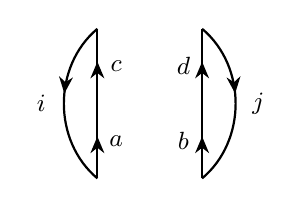
\begin{tikzpicture}[gdiag]\gbox{4}
  \draw[gpart] (0,0) -- (0,1); \draw[gpart] (0,1) -- (0,2);
  \draw[gpart] (1.4,0) -- (1.4,1); \draw[gpart] (1.4,1) -- (1.4,2);
  \draw[ghole] (0,0) to[bend left=50] (0,2);
  \draw[ghole] (1.4,0) to[bend right=50] (1.4,2);
  \gv{0}{1.4}{0} \gv{0}{1.4}{1} \gv{0}{1.4}{2}
  \node[glab] at (-0.75,1) {$i$}; \node[glab] at (2.15,1) {$j$};
  \node[glab] at (0.25,0.5) {$a$}; \node[glab] at (1.15,0.5) {$b$};
  \node[glab] at (0.25,1.5) {$c$}; \node[glab] at (1.15,1.5) {$d$};
\end{tikzpicture}
\\
% ---- 5: hole-hole ladder
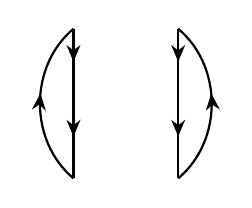
\begin{tikzpicture}[gdiag]\gbox{5}
  \draw[ghole] (0,0) -- (0,1); \draw[ghole] (0,1) -- (0,2);
  \draw[ghole] (1.4,0) -- (1.4,1); \draw[ghole] (1.4,1) -- (1.4,2);
  \draw[gpart] (0,0) to[bend left=50] (0,2);
  \draw[gpart] (1.4,0) to[bend right=50] (1.4,2);
  \gv{0}{1.4}{0} \gv{0}{1.4}{1} \gv{0}{1.4}{2}
\end{tikzpicture}
&
% ---- 6: three one-body vertices, insertion on the particle line
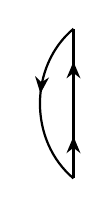
\begin{tikzpicture}[gdiag]\gbox{6}
  \draw[gpart] (0,0) -- (0,1); \draw[gpart] (0,1) -- (0,2);
  \draw[ghole] (0,0) to[bend left=50] (0,2);
  \gx{0}{1.4}{0} \gx{0}{1.4}{1} \gx{0}{1.4}{2}
\end{tikzpicture}
&
% ---- 7: three one-body vertices, insertion on the hole line
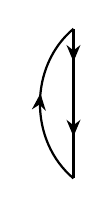
\begin{tikzpicture}[gdiag]\gbox{7}
  \draw[ghole] (0,0) -- (0,1); \draw[ghole] (0,1) -- (0,2);
  \draw[gpart] (0,0) to[bend left=50] (0,2);
  \gx{0}{1.4}{0} \gx{0}{1.4}{1} \gx{0}{1.4}{2}
\end{tikzpicture}
&
% ---- 8: one-body vertex on a hole line of the second-order diagram
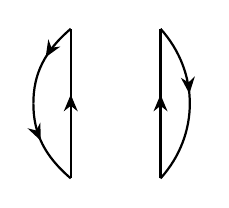
\begin{tikzpicture}[gdiag]\gbox{8}
  \draw[ghole] (0.4,0) .. controls (0.05,0.3) and (-0.1,0.6) .. (-0.1,1);
  \draw[ghole] (-0.1,1) .. controls (-0.1,1.4) and (0.05,1.7) .. (0.4,2);
  \draw[gpart] (0.4,0) -- (0.4,2);
  \draw[gpart] (1.6,0) -- (1.6,2);
  \draw[ghole] (1.6,0) to[bend right=42] (1.6,2);
  \gv{0.4}{1.6}{0} \gv{0.4}{1.6}{2} \gx{-0.1}{-0.95}{1}
\end{tikzpicture}
\\
% ---- 9: one-body vertex on a particle line of the second-order diagram
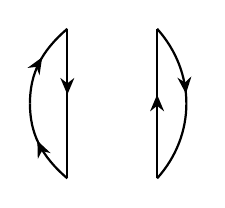
\begin{tikzpicture}[gdiag]\gbox{9}
  \draw[gpart] (0.4,0) .. controls (0.05,0.3) and (-0.1,0.6) .. (-0.1,1);
  \draw[gpart] (-0.1,1) .. controls (-0.1,1.4) and (0.05,1.7) .. (0.4,2);
  \draw[ghole] (0.4,0) -- (0.4,2);
  \draw[gpart] (1.6,0) -- (1.6,2);
  \draw[ghole] (1.6,0) to[bend right=42] (1.6,2);
  \gv{0.4}{1.6}{0} \gv{0.4}{1.6}{2} \gx{-0.1}{-0.95}{1}
\end{tikzpicture}
&
% ---- 10: one-body vertex on top, particle line through the middle vertex
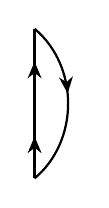
\begin{tikzpicture}[gdiag]\gbox{10}
  \gl{0}{0}{1}
  \draw[gpart] (1.4,0) -- (1.4,1); \draw[gpart] (1.4,1) -- (1.4,2);
  \draw[ghole] (1.4,0) to[bend right=50] (1.4,2);
  \gv{0}{1.4}{0} \gv{0}{1.4}{1} \gx{1.4}{0}{2}
\end{tikzpicture}
&
% ---- 11: one-body vertex on top, hole line through the middle vertex
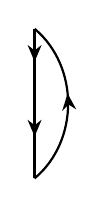
\begin{tikzpicture}[gdiag]\gbox{11}
  \gl{0}{0}{1}
  \draw[ghole] (1.4,0) -- (1.4,1); \draw[ghole] (1.4,1) -- (1.4,2);
  \draw[gpart] (1.4,0) to[bend right=50] (1.4,2);
  \gv{0}{1.4}{0} \gv{0}{1.4}{1} \gx{1.4}{0}{2}
\end{tikzpicture}
&
% ---- 12: one-body vertex at the bottom, particle line through the middle vertex
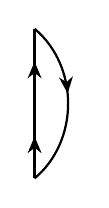
\begin{tikzpicture}[gdiag]\gbox{12}
  \gl{0}{1}{2}
  \draw[gpart] (1.4,0) -- (1.4,1); \draw[gpart] (1.4,1) -- (1.4,2);
  \draw[ghole] (1.4,0) to[bend right=50] (1.4,2);
  \gx{1.4}{0}{0} \gv{0}{1.4}{1} \gv{0}{1.4}{2}
\end{tikzpicture}
\\
% ---- 13: one-body vertex at the bottom, hole line through the middle vertex
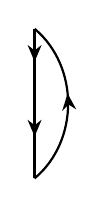
\begin{tikzpicture}[gdiag]\gbox{13}
  \gl{0}{1}{2}
  \draw[ghole] (1.4,0) -- (1.4,1); \draw[ghole] (1.4,1) -- (1.4,2);
  \draw[gpart] (1.4,0) to[bend right=50] (1.4,2);
  \gx{1.4}{0}{0} \gv{0}{1.4}{1} \gv{0}{1.4}{2}
\end{tikzpicture}
&
% ---- 14: one-body, two-body, one-body
\begin{tikzpicture}[gdiag]\gbox{14}
  \gl{0.2}{0}{1} \gl{1.0}{1}{2}
  \gx{0.2}{-0.6}{0} \gv{0.2}{1.0}{1} \gx{1.0}{1.8}{2}
\end{tikzpicture}
&
% ---- 15: one-body, one-body, two-body
\begin{tikzpicture}[gdiag]\gbox{15}
  \gl{0.2}{0}{2} \gl{1.0}{1}{2}
  \gx{0.2}{-0.6}{0} \gx{1.0}{1.8}{1} \gv{0.2}{1.0}{2}
\end{tikzpicture}
&
% ---- 16: two-body, one-body, one-body
\begin{tikzpicture}[gdiag]\gbox{16}
  \gl{0.2}{0}{1} \gl{1.0}{0}{2}
  \gv{0.2}{1.0}{0} \gx{0.2}{-0.6}{1} \gx{1.0}{1.8}{2}
\end{tikzpicture}
\end{tabular}
\caption{All diagrams (so-called anti-symmetrized Goldstone diagrams)
  to third order in the perturbation for the ground-state energy. The
  first-order term is excluded. Time runs upwards; a line with an
  arrow pointing upwards is a particle line and a line with an
  arrow pointing downwards is a hole line. A dashed line between two dots is
  the two-body interaction and represents an anti-symmetrized matrix
  element. A dashed line which ends in a cross is the one-body vertex
  $\tilde{f}_{pq}$ of Eq.~(\ref{eq:onebodyvertex}), which contains the
  contribution from the Hartree-Fock potential. Diagrams 1 and 2 are
  of second order, diagrams 3--16 of third order. The labels in diagram 4
  indicate our convention, $i,j,\dots$ for hole states and $a,b,\dots$ for
  particle states.\label{fig:diagrams}}
\end{figure}

\item (15/100 points) \textbf{The wave operator to first order and the exact
  diagonalization.}
Diagram 1 in Fig.~\ref{fig:diagrams} represents a second-order
contribution to the energy and a so-called $2p-2h$ contribution to the
intermediate states.
\begin{enumerate}
\item Write down the expression for the wave operator to first order
  acting on the reference state,
  $\hat{\Omega}^{(1)}|\Phi_0\rangle$, in terms of the single-particle
  energies, the two-body matrix elements and the one-body vertex
  $\tilde{f}_{pq}$ defined in Eq.~(\ref{eq:onebodyvertex}) of Part II,
  and draw the diagrams which represent it. For the pairing model,
  which Slater determinants enter, and what are their amplitudes
  $t_i^a=\langle\Phi_i^a|\hat{\Omega}^{(1)}|\Phi_0\rangle$ as functions
  of $g$?
\item Compare these amplitudes, for $g\in[-1,1]$, with the
  coefficients of the same Slater determinants in the ground state of
  the configuration interaction calculation with at most $2p2h$
  excitations (exercise 3 of the first midterm), and in the exact
  ground state from the diagonalization of the matrix in
  Eq.~(\ref{eq:hmatrix}) (exercise 2 of the first midterm). In order to
  compare, the eigenvectors must be brought to intermediate
  normalization, that is, divided by the coefficient of
  $|\Phi_0\rangle$. Plot the amplitudes as functions of $g$ and
  comment your results for various values of $g\in[-1,1]$. Which
  contributions are contained in the configuration interaction
  coefficients but not in the wave operator to first order?
\item The Slater determinant $|\Phi_{12}^{34}\rangle=|0011\rangle$ does
  not appear to first order. Use
  $\hat{\Omega}^{(2)}|\Phi_0\rangle$ from exercise 1 to find its
  amplitude to second order in the interaction, and show that it
  equals
\[
\langle\Phi_{12}^{34}|\hat{\Omega}^{(2)}|\Phi_0\rangle
=t_1^3t_2^4+t_1^4t_2^3 ,
\]
  a sum of products of first-order amplitudes. Compare with the exact
  coefficient of $|0011\rangle$ for $g\in[-1,1]$ and comment.
\item Compute the expectation value of $\hat{H}$ in the normalized
  state
  $|\Phi_0\rangle+\hat{\Omega}^{(1)}|\Phi_0\rangle$ and show that it
  can be written as
\[
E_{\mathrm{ref}}+\frac{E^{(2)}+E^{(3)}}
{1+\langle\Psi^{(1)}|\Psi^{(1)}\rangle} .
\]
  Compare it with the exact energy for $g\in[-1,1]$. Is it an upper
  bound to the exact energy? Is it the same as the energy through
  third order, and to which order in $g$ does it agree with the exact
  energy?
\end{enumerate}
\end{enumerate}

%======================================================================
\subsection*{Part II: Diagrams to third order and the role of Hartree-Fock (35 points)}

We now study the system using non-degenerate Rayleigh-Schr\"odinger
perturbation theory to third order in the perturbation, in its
diagrammatic form. With
$\hat{H}_0=\sum_p\varepsilon_pa^\dagger_pa_p$ as the unperturbed
Hamiltonian and with the perturbation $\hat{V}=\hat{H}-\hat{H}_0$
written in normal-ordered form with respect to $|\Phi_0\rangle$,
\[
\hat{V}=E^{(1)}+\sum_{pq}\tilde{f}_{pq}\normord{a^\dagger_pa_q}
+\frac{1}{4}\sum_{pqrs}\langle pq|V|rs\rangle
\normord{a^\dagger_pa^\dagger_qa_sa_r},
\]
the diagrams are built from a two-body vertex and the one-body vertex
\begin{equation}
\tilde{f}_{pq}=\langle p|h_0|q\rangle-\varepsilon_p\delta_{pq}
+\sum_{j}\langle pj|V|qj\rangle ,
\label{eq:onebodyvertex}
\end{equation}
where the sum over $j$ runs over the hole states. The last term is the
Hartree-Fock potential. The first two terms cancel each other when
the single-particle states are eigenstates of $\hat{h}_0$ with
eigenvalues $\varepsilon_p$, as in the definition of our model. If we
exclude the first-order contribution, all possible diagrams to third
order are shown in Fig.~\ref{fig:diagrams}.

\begin{enumerate}
\setcounter{enumi}{2}

\item (20/100 points) \textbf{The energy to third order for the pairing model.}
\begin{enumerate}
\item Use the diagram rules from the lectures to write down the
  algebraic expressions for diagrams 1, 3, 4, 5, 8 and 9 of
  Fig.~\ref{fig:diagrams} for a general Hamiltonian. Explain for each
  of them the energy denominators, the numerical factor and the sign.
\item Compute the one-body vertex $\tilde{f}_{pq}$ of
  Eq.~(\ref{eq:onebodyvertex}) for the pairing model, for hole states
  and for particle states. Based on the form of the interaction, which
  of the sixteen diagrams contribute to the energy of the ground
  state? Go through all the diagrams (or groups of diagrams) and
  explain why they vanish or not.
\item Write down the expressions for the diagrams that contribute for
  our system of four particles in four levels, and find their
  contributions as functions of $g$. Give the result for each diagram
  separately, and give the corrections $E^{(2)}$ and $E^{(3)}$ and the
  energy through third order.
\item In exercise 1 the third-order correction was written as
  $E^{(3)}=\langle\hat{V}\hat{R}\hat{V}\hat{R}\hat{V}\rangle
  -E^{(1)}\langle\hat{V}\hat{R}^2\hat{V}\rangle$.
  Evaluate the two terms with the matrix in Eq.~(\ref{eq:hmatrix}) and
  show that their sum agrees with the sum of the third-order
  diagrams. Show that the second term cancels the part of the first
  term which comes from the diagonal matrix elements
  $\langle\Phi_i^a|\hat{V}|\Phi_i^a\rangle$. Which diagram, and which
  parts of the other diagrams, have the same values as these two
  pieces? Explain the cancellation in terms of the diagrams. Would you
  expect the second term to be equal to one particular diagram for any
  Hamiltonian and any choice of $\hat{H}_0$? Comment your results.
\end{enumerate}
A numerical comparison with the results of the first midterm follows
in exercise 6.

\item (15/100 points) \textbf{Hartree-Fock and the diagrams of perturbation theory.}
In this exercise you are asked to explain how a Hartree-Fock
calculation affects the diagrams of perturbation theory, and why some
of them become zero.
\begin{enumerate}
\item Consider first a general Hamiltonian. Recall the normal-ordered
  Hamiltonian and the Hartree-Fock equations
  $\hat{h}^{\mathrm{HF}}|p\rangle=\varepsilon^{\mathrm{HF}}_p|p\rangle$
  from the first midterm. Draw the one-body vertex of
  Eq.~(\ref{eq:onebodyvertex}) as a sum of diagrams. Show that if the
  single-particle states are the Hartree-Fock states and the
  unperturbed Hamiltonian is
  $\hat{H}_0^{\mathrm{HF}}=\sum_p\varepsilon_p^{\mathrm{HF}}a^\dagger_pa_p$,
  then $\tilde{f}_{pq}=0$ for all $p$ and $q$. Which diagrams in
  Fig.~\ref{fig:diagrams} are then left? Explain in words what the
  Hartree-Fock calculation has done with the contributions that the
  other diagrams represent. Which of the diagrams vanish already
  because of Brillouin's theorem, $\tilde{f}_{ai}=0$, that is, if we
  use Hartree-Fock single-particle states but keep an unperturbed
  Hamiltonian whose single-particle energies are not the Hartree-Fock
  ones?
\item For the pairing model the Hartree-Fock single-particle states
  are the original ones, but the Hartree-Fock single-particle energies
  in Eq.~(\ref{eq:hfenergies}) differ from $\varepsilon_p=p-1$. We
  thus have two ways of dividing the same Hamiltonian into an
  unperturbed part and a perturbation: the original one, used in
  exercise 3, and the Hartree-Fock one,
  $\hat{H}=\hat{H}_0^{\mathrm{HF}}+\hat{V}^{\mathrm{HF}}$. Find
  $E^{(0)}_0$ and $E^{(1)}$ for the two choices. Does the energy
  through first order depend on the choice? Which of the diagrams that
  contributed in exercise 3 are zero with the Hartree-Fock choice, and
  what has changed in the remaining ones? Write down the second-order
  correction $E^{(2)}_{\mathrm{HF}}$ with the Hartree-Fock choice as
  function of $g$.
\item With the Hartree-Fock choice the unperturbed Hamiltonian depends
  on $g$. A correction of order $n$ in the perturbation
  $\hat{V}^{\mathrm{HF}}$ is therefore not proportional to $g^n$, and
  the order in the perturbation must be distinguished from the power
  of $g$. Expand $E^{(2)}_{\mathrm{HF}}$ in powers of $g$ and show that
  the terms proportional to $g^2$ and $g^3$ reproduce diagram 1 and
  diagram 8 of exercise 3, and that the expansion continues with an
  infinite series of higher powers of $g$. Draw one of the diagrams
  of order $g^4$ of this series and explain how the series has been
  summed. Explain why the energies through third order obtained with
  the two choices must have the same coefficients of $g^2$ and $g^3$
  when they are expanded in powers of $g$, while they differ as
  numbers for a given value of $g$. Does this tell us which of the two
  choices is the more accurate one at a given order?
\end{enumerate}

\end{enumerate}

%======================================================================
\subsection*{Part III: How to compute diagrams (30 points)}

\begin{enumerate}
\setcounter{enumi}{4}

\item (15/100 points) \textbf{Slater determinant basis and single-particle basis.}
The contributions to the energy can be computed either in the basis of
Slater determinants or directly in the single-particle basis. In
this exercise you should explain how each of them is done efficiently.
\begin{enumerate}
\item \emph{Slater determinant basis.} Let $m,n\neq 0$ label the
  Slater determinants other than the reference state, and define the
  vector $\bm{w}$ with elements
  $w_m=\langle\Phi_m|\hat{V}|\Phi_0\rangle$, the matrix $\bm{W}$ with
  elements
  $W_{mn}=\langle\Phi_m|\hat{V}|\Phi_n\rangle-E^{(1)}\delta_{mn}$ and
  the diagonal matrix $\bm{R}$ with elements
  $R_{mn}=\delta_{mn}/D_m$. Show that Eq.~(\ref{eq:e2e3}) becomes
\[
E^{(2)}=\bm{w}^\dagger\bm{R}\,\bm{w},\qquad
E^{(3)}=\bm{w}^\dagger\bm{R}\,\bm{W}\bm{R}\,\bm{w},
\]
  and explain how the recursion relations in
  Eq.~(\ref{eq:recursion}) give the corrections of any order with
  matrix-vector multiplications only. Read off $\bm{w}$, $\bm{W}$ and
  $\bm{R}$ for the pairing model from Eq.~(\ref{eq:hmatrix}) and compute
  $E^{(2)}$ and $E^{(3)}$ by hand. What are the diagonal elements
  $W_{mm}$ for the four $2p2h$ states, and how is this related to
  what you found in exercise 3(iv)? How does the number of Slater
  determinants grow with the number of levels $L$ and the number of
  particles, with and without broken pairs?
\item \emph{Single-particle basis.} For larger systems the basis of
  Slater determinants cannot be set up, and the diagrams are evaluated
  directly as sums over single-particle states. Define the matrix
  $\bm{V}_{hhpp}$, whose rows are labelled by pairs $(ij)$ of hole
  states and whose columns are labelled by pairs $(ab)$ of particle
  states, and the matrix of amplitudes $\bm{T}$,
\[
\left[\bm{V}_{hhpp}\right]_{(ij),(ab)}=\langle ij|V|ab\rangle,\qquad
\left[\bm{T}\right]_{(ab),(ij)}
=\frac{\langle ab|V|ij\rangle}{D_{ij}^{ab}} ,
\]
  where the indices are spin-orbitals and, to begin with, all ordered
  pairs are included, that is both $(ij)$ and $(ji)$. Show that
  diagram 1 in Fig.~\ref{fig:diagrams} can be written as a trace over
  a product of matrices, as discussed in the lectures of week 45,
\begin{equation}
\text{diagram 1}=\frac{1}{4}\operatorname{Tr}\left(\bm{V}_{hhpp}\bm{T}\right).
\label{eq:e2trace}
\end{equation}
  This is the complete second-order correction $E^{(2)}$ only when
  diagram 2 vanishes. Write down the expression for diagram 2, which
  has to be added in the general case. What happens with the factor
  $1/4$ if only one ordering of each pair is kept, $i<j$ and $a<b$?
  Define in the same way the matrices $\bm{V}_{pppp}$ and
  $\bm{V}_{hhhh}$ and write diagrams 4 and 5 as traces over products
  of three matrices, using $\bm{T}$ and its Hermitian conjugate
  $\bm{T}^\dagger$. If $n_h$ is the number of hole states and $n_p$
  the number of particle states, how does the number of operations
  needed for diagrams 1, 4 and 5 grow with $n_h$ and $n_p$? Note that
  a trace needs only the diagonal elements of a product. Compare with
  the growth of the number of Slater determinants. What is gained, and
  what is not gained, by writing the diagrams as products of matrices?
\item \emph{Symmetries.} For the pairing model only very few of the
  two-body matrix elements are different from zero. Show that the
  matrices above reduce to matrices whose rows and columns are
  labelled by the levels $i\in\{1,2\}$ and $a\in\{3,4\}$ of a pair,
  write down $\bm{V}_{hhpp}$, $\bm{V}_{pppp}$, $\bm{V}_{hhhh}$ and
  $\bm{T}$ in this form, and compute diagrams 1, 4 and 5 by hand as
  traces. What has happened with the factors $1/4$ and $1/8$? For a
  general two-body interaction, how can the conserved quantum numbers
  of a pair of single-particle states be used to divide the matrices
  into smaller blocks?
\end{enumerate}
If time permits, explain why diagram 3 cannot be written in terms of
the matrices above, and how the two-body matrix elements have to be
reorganized in order to write it as a trace over a product of matrices
as well. This last part is not required for full score.

\item (15/100 points) \textbf{A program for the energy to second and third order.}
Write a program (in Python, C++ or Fortran) which computes the
corrections $E^{(2)}$ and $E^{(3)}$, and from them the ground-state
energy through second and through third order, for the pairing model
with four particles in four levels, as function of the strength
$g\in[-1,1]$ of the interaction. The programs \texttt{mbpt.py} and
\texttt{diagrams.py} in
\texttt{doc/BookManybody/BookPrograms/chapter09/} and the notebook
\texttt{doc/LectureNotes/mbptheory.ipynb} may be consulted, but you
are expected to write and to explain your own program.
\begin{enumerate}
\item Implement both approaches of exercise 5: the recursion relations
  in the basis of Slater determinants, starting from the matrix in
  Eq.~(\ref{eq:hmatrix}), and the diagrams in the single-particle
  basis, either as sums over single-particle states or as products
  of matrices. Check that the two give the same $E^{(2)}$ and
  $E^{(3)}$, and that they agree with your analytical results from
  exercise 3.
\item Compare with the exact diagonalization of exercise 2 of the
  first midterm. Plot, as functions of $g$, the reference energy, the
  energy through second order, the energy through third order and the
  exact energy. Plot also the absolute deviations
  $|E-E_{\mathrm{FCI}}|$ from the exact energy on a logarithmic scale,
  leaving out $g=0$, where all deviations vanish. Comment your
  results. For which values of $g$ is the deviation of the energy
  through third order smaller than $10^{-3}$, and how large is it
  compared with the correlation energy at $|g|=0.5$ and $|g|=1$? Does
  the third-order correction improve the result for all
  $g\in[-1,1]$? Are the perturbative energies above or below the
  exact energy, and is there a difference between an attractive
  ($g>0$) and a repulsive ($g<0$) interaction?
\item Repeat the calculation with the Hartree-Fock single-particle
  energies of exercise 4 in the unperturbed Hamiltonian. Remember
  that the energy through first order is the same for the two
  choices. Compare the two choices with the exact result for $g>0$
  and for $g<0$, and describe what you observe. Try to explain it by
  looking at the energy denominators and at the diagonal elements
  $W_{mm}$ of exercise 5 for the two choices.
\end{enumerate}
If time permits, use the recursion relations to compute the
corrections of higher orders and study how the perturbation series
behaves as function of $g$, also for $|g|>1$, or extend your program
to more levels and particles, for example eight levels and four
pairs. This last part is not required for full score.

\end{enumerate}

%======================================================================
\subsection*{Part IV: Comparison with the first midterm (10 points)}

\begin{enumerate}
\setcounter{enumi}{6}

\item (10/100 points) \textbf{Comparison with FCI, Hartree-Fock and the DMRG.}
Collect, in one figure and in a table for some selected values of the
strength (for example $g=\pm 0.5$ and $g=\pm 1$), the ground-state
energies from both midterms. All energies must refer to the same
system: four particles in four levels with $\xi=1$ and no broken
pairs. For the matrix product states and the DMRG you should check
that your states have four particles.
\begin{itemize}
\item The Hartree-Fock energy (exercise 4 of the first midterm), the
  configuration interaction calculation with at most $2p2h$
  excitations (exercise 3) and the exact FCI energy (exercise 2).
\item The energies of the matrix product states with bond dimension
  $\chi=1$ and $\chi=2$, and your DMRG results if you computed them
  (exercise 8 of the first midterm).
\item The energies through second and through third order in
  perturbation theory, with the original and with the Hartree-Fock
  single-particle energies (exercises 3, 4 and 6 of this midterm).
\end{itemize}
Plot also the absolute deviations from the exact energy on a
logarithmic scale, as in exercise 6; you may reuse your figures from
exercise 6 and add the results of the first midterm to them. Discuss
your results. You should at least address the following questions:
\begin{enumerate}
\item How much of the correlation energy
  $E_{\mathrm{FCI}}-E_{\mathrm{HF}}$ does each method recover, and how
  does this depend on $g$?
\item Which of the methods are variational, that is, which of them
  give an upper bound to the exact ground-state energy of this system
  for every $g$, and which do not? Are your numbers in agreement with
  this?
\item Which quantity controls the accuracy of each method (the order
  in the perturbation, the number of Slater determinants, the bond
  dimension $\chi$), and how does the computational cost grow with the
  number of levels and particles when this quantity is increased? Is
  the accuracy guaranteed to improve when it is increased?
\item Consider two copies of the system which do not interact with
  each other. For which of the methods is the energy of the two
  copies together equal to the sum of the energies of the two copies
  computed separately? Discuss Hartree-Fock, the exact
  diagonalization, the configuration interaction calculation with at
  most $2p2h$ excitations of the combined system, each order of
  Rayleigh-Schr\"odinger perturbation theory, and a matrix product
  state with a given bond dimension when the levels of the two copies
  are placed after each other on the chain. How is your answer for
  perturbation theory related to the linked-diagram theorem discussed
  in the lectures? You may answer with arguments only, or support
  them with a numerical test.
\item Which method would you choose for a system with many levels and
  weak pairing, and which for strong pairing, $|g|>1$? Base your
  answer on what you have observed in the two midterms.
\end{enumerate}

If time permits, compute the entanglement entropy of the middle cut
(see exercise 8 of the first midterm) for the normalized wave function
to first order of exercise 2 and compare it with the entropy of the
exact ground state. This last part is not required for full score.

\end{enumerate}



 \end{document}
